% !TeX program = pdflatex
% !TeX encoding = UTF-8
\documentclass[aspectratio=169,12pt]{beamer}
% aspectratio=169 cho màn hình rộng, có thể đổi thành 43 cho màn hình vuông

% Preamble for Beamer presentation (Vietnamese)
% Engine: pdfLaTeX hoặc XeLaTeX

% Beamer class với theme và color scheme
\usetheme{Warsaw}
\usecolortheme{whale}
\useinnertheme{rounded}
\useoutertheme{infolines}

% Custom color scheme
\definecolor{mainblue}{RGB}{0,51,102}
\definecolor{accentblue}{RGB}{0,102,204}
\definecolor{mainred}{RGB}{204,0,51}
\definecolor{maingreen}{RGB}{0,128,0}
\setbeamercolor{structure}{fg=mainblue}
\setbeamercolor{block title}{bg=mainblue,fg=white}
\setbeamercolor{block body}{bg=blue!5,fg=black}
\setbeamercolor{alerted text}{fg=mainred}

% Font encoding cho tiếng Việt
\usepackage{iftex}
\ifPDFTeX
  \usepackage[T5]{fontenc}
  \usepackage[utf8]{inputenc}
  \usepackage[vietnamese]{babel}
  \usepackage{vntex}
\else
  \usepackage{fontspec}
  \defaultfontfeatures{Ligatures=TeX}
  \setmainfont{Times New Roman}
  \setsansfont{Arial}
  \setmonofont{Consolas}
\fi

% Math packages
\usepackage{amsmath,amssymb,mathtools}

% Graphics
\usepackage{graphicx}
\graphicspath{{assets/figures/}}

% Tables
\usepackage{booktabs}
\usepackage{array}
\usepackage{multirow}

% Colors
\usepackage{xcolor}

% Hyperref
\usepackage{hyperref}
\hypersetup{
  colorlinks=true,
  linkcolor=blue!60!black,
  urlcolor=blue!60!black
}

% TikZ for diagrams
\usepackage{tikz}
\usetikzlibrary{arrows.meta,positioning}

% Caption settings
\usepackage{caption}
\captionsetup{font=small,labelfont=bf}


% Beamer specific settings
\setbeamertemplate{navigation symbols}{} % Remove navigation symbols
\setbeamertemplate{footline}[frame number] % Show frame numbers

% Spacing improvements
\setlength{\parskip}{0.5em}
\setbeamersize{text margin left=1em,text margin right=1em}

% Item spacing
\setlength{\leftmargini}{1.5em}
\setlength{\itemindent}{0.5em}

% Title page info (sẽ được override trong presentation.tex)
\title{Nghiên cứu các yếu tố ảnh hưởng đến quyết định nghỉ việc của nhân viên}
\subtitle{Tiếp cận bằng mô hình Hồi quy Logistic}
\author{Nguyễn Thị Quỳnh Mai}
\date{\today}

% Vietnamese labels for Beamer
\setbeamertemplate{caption}[numbered]



% Title information
\title[Nghiên cứu Nghỉ việc NV]{Nghiên cứu các yếu tố ảnh hưởng đến quyết định nghỉ việc của nhân viên}
\subtitle{Tiếp cận bằng mô hình Hồi quy Logistic}
\author[N.T.Q. Mai]{Nguyễn Thị Quỳnh Mai}
\date{\today}

\begin{document}

% Title slide
\begin{frame}
  \titlepage
\end{frame}

% Outline
\begin{frame}{Nội dung trình bày}
  \tableofcontents
\end{frame}

% Sections
\section{Tổng quan}
% Overview slides
\begin{frame}{Tổng quan nghiên cứu}
  \Large \textbf{Employee Attrition} (Nghỉ việc)
  
  \vspace{0.4cm}
  \textbf{Mục tiêu:}
  \begin{itemize}
    \item Dự đoán xác suất nhân viên nghỉ việc
    \item Diễn giải các yếu tố ảnh hưởng bằng Odds Ratio
  \end{itemize}
  
  \vspace{0.4cm}
  \textbf{Phương pháp:}
  \begin{itemize}
    \item \textbf{Logistic Regression} (sklearn) cho dự đoán
    \item \textbf{Logit} (statsmodels) cho suy luận thống kê
  \end{itemize}
  
  \vspace{0.4cm}
  \textbf{Dữ liệu:} 1{,}470 quan sát, tỷ lệ nghỉ việc: \textbf{16.12\%}

  \vspace{0.4cm}
  \small Toàn bộ mã nguồn và báo cáo được lưu trong kho lưu trữ:
  \texttt{https://github.com/ti014/hr-employee-attrition-analysis.git}
\end{frame}

\begin{frame}{Kết quả chính - Hiệu năng mô hình}
  \textbf{Hiệu năng mô hình:}
  
  \vspace{0.3cm}
  \begin{itemize}
    \item \textcolor{accentblue}{\textbf{ROC AUC}}: \Large \textbf{0.8031}
    \item \textcolor{accentblue}{\textbf{Recall}}: \Large \textbf{0.6383} (phát hiện 64\% nhân sự nghỉ việc)
    \item Accuracy: 0.7517
    \item Precision: 0.3488
    \item F1: 0.4511
  \end{itemize}
  
  \vspace{0.4cm}
  \begin{alertblock}{}
    Mô hình dự đoán vượt trội baseline, phân biệt được phần lớn nhân sự nguy cơ cao (AUC > 80\%).
  \end{alertblock}
\end{frame}

\begin{frame}{Kết quả chính - Yếu tố nổi bật}
  \textbf{Yếu tố ảnh hưởng nổi bật:}
  
  \vspace{0.3cm}
  \begin{itemize}
    \item \textcolor{mainred}{$\uparrow$ \textbf{OverTime\_Yes}}: làm tăng mãnh liệt xác suất nghỉ việc
    \item \textcolor{mainred}{$\uparrow$ \textbf{JobRole\_Sales Representative}}: có rủi ro nghỉ việc đặc biệt cao
    \item \textcolor{maingreen}{$\downarrow$ \textbf{EnvironmentSatisfaction}}: tỷ lệ nghịch với khả năng nghỉ việc, bảo vệ mạnh
    \item \textcolor{maingreen}{$\downarrow$ \textbf{JobInvolvement}}: sự gắn kết bảo vệ nhân sự
  \end{itemize}
\end{frame}


\section{Dữ liệu và phương pháp}
% Data and Methodology slides
\begin{frame}{Dữ liệu}
  \textbf{Dataset:} \texttt{WA\_Fn-UseC\_-HR-Employee-Attrition.csv} với 1{,}470 quan sát
  
  \vspace{0.4cm}
  \textbf{Biến phân loại chính:}
  \begin{itemize}
    \item OverTime, JobRole, BusinessTravel, MaritalStatus
  \end{itemize}
  
  \vspace{0.4cm}
  \textbf{Biến số tiêu biểu:}
  \begin{itemize}
    \item Age, MonthlyIncome, YearsAtCompany
    \item EnvironmentSatisfaction, JobInvolvement, DistanceFromHome
  \end{itemize}
  
  \vspace{0.4cm}
  \textbf{Biến mục tiêu:} \texttt{Attrition} (1 = Nghỉ việc, 0 = Ở lại)
\end{frame}

\begin{frame}{Dữ liệu - Lưu ý}
  \begin{alertblock}{Lưu ý}
    Tỷ lệ nghỉ việc 16.12\% $\Rightarrow$ mất cân bằng lớp (class imbalance) $\Rightarrow$ dùng \texttt{class\_weight='balanced'}
  \end{alertblock}
  
  \vspace{0.4cm}
  \textbf{Ý nghĩa:}
  \begin{itemize}
    \item Dataset chỉ có khoảng 16\% nhân viên nghỉ việc thực tế
    \item Thuật toán LR dễ bị thiên hướng luôn dự đoán "Không nghỉ việc"
    \item \texttt{class\_weight='balanced'} giúp mô hình học nhạy cảm hơn đối lưu các phần tử thiểu số
  \end{itemize}
\end{frame}

\begin{frame}{Logistic Regression - Bài toán và Công thức}
  \textbf{Bài toán:} Tính xác suất một nhân viên sẽ đưa ra quyết định nghỉ việc (Attrition = 1).
  
  \vspace{0.2cm}
  \textbf{Công thức xác suất Sigmoid:}
  \[
  p(y=1\mid x) = \frac{1}{1+e^{-z}}, \quad \text{với } z = \beta_0 + \beta_1 x_1 + \dots + \beta_d x_d
  \]
  
  \textbf{Tính toán từng phần tử để thay vào công thức:}
  \begin{itemize}
    \item \textbf{$p(y=1\mid x)$:} Kết quả đầu ra (xác suất làm tròn nội suy từ 0 đến 1).
    \item \textbf{Biến hệ $x_i$:} Giá trị đặc trưng của nhân viên (VD: $x_1$ = Age, $x_2$ = OverTime=Yes).
    \item \textbf{Trọng số $\beta_i$:} Mức độ tác động của đặc trưng (Do thuật toán tính toán).
    \item \textbf{Tính $z$:} Nhân thực tế từng giá trị $x_i$ của nhân viên đó với hệ số $\beta_i$, rồi lấy tổng cộng với hệ số tự do $\beta_0$.
    \item \textbf{Toán hạng hàm mũ $e$:} Thế $z$ vào $1+e^{-z}$ ở mẫu số để ánh xạ kết quả $z$ tuyến tính thành một xác suất toán học.
  \end{itemize}
\end{frame}

\begin{frame}{Hàm mục tiêu và Regularization}
  \textbf{Hàm mục tiêu:} Âm log-likelihood (NLL) kết hợp L2 regularization 
  \[
  \mathcal{L}(\beta) = -\sum_{i=1}^{n}\Big[y_i\log p_i + (1-y_i)\log(1-p_i)\Big] + \lambda \|\beta\|_2^2
  \]
  
  \vspace{0.4cm}
  \begin{itemize}
    \item Regularization ngăn hệ số mô hình bùng nổ, dễ xử lý các biến số đo lường đơn vị lớn.
  \end{itemize}
  
  \vspace{0.3cm}
  \begin{alertblock}{Thiết kế Split \& Tiền Xử Lý}
    \begin{itemize}
      \item Train/Test theo stratified 80/20 nhằm đảm bảo phân bố 16\% xuyên suốt.
      \item sklearn: Pipeline (OneHotEncoder + StandardScaler) phục vụ hệ thống máy học tốc độ cao.
      \item statsmodels: Cung cấp p-value và tính Odds Ratio giải thích chuyên sâu.
    \end{itemize}
  \end{alertblock}
\end{frame}


\section{Kết quả EDA}
% EDA slides
\begin{frame}{Tỷ lệ nghỉ việc theo OverTime}
  \begin{figure}
    \centering
    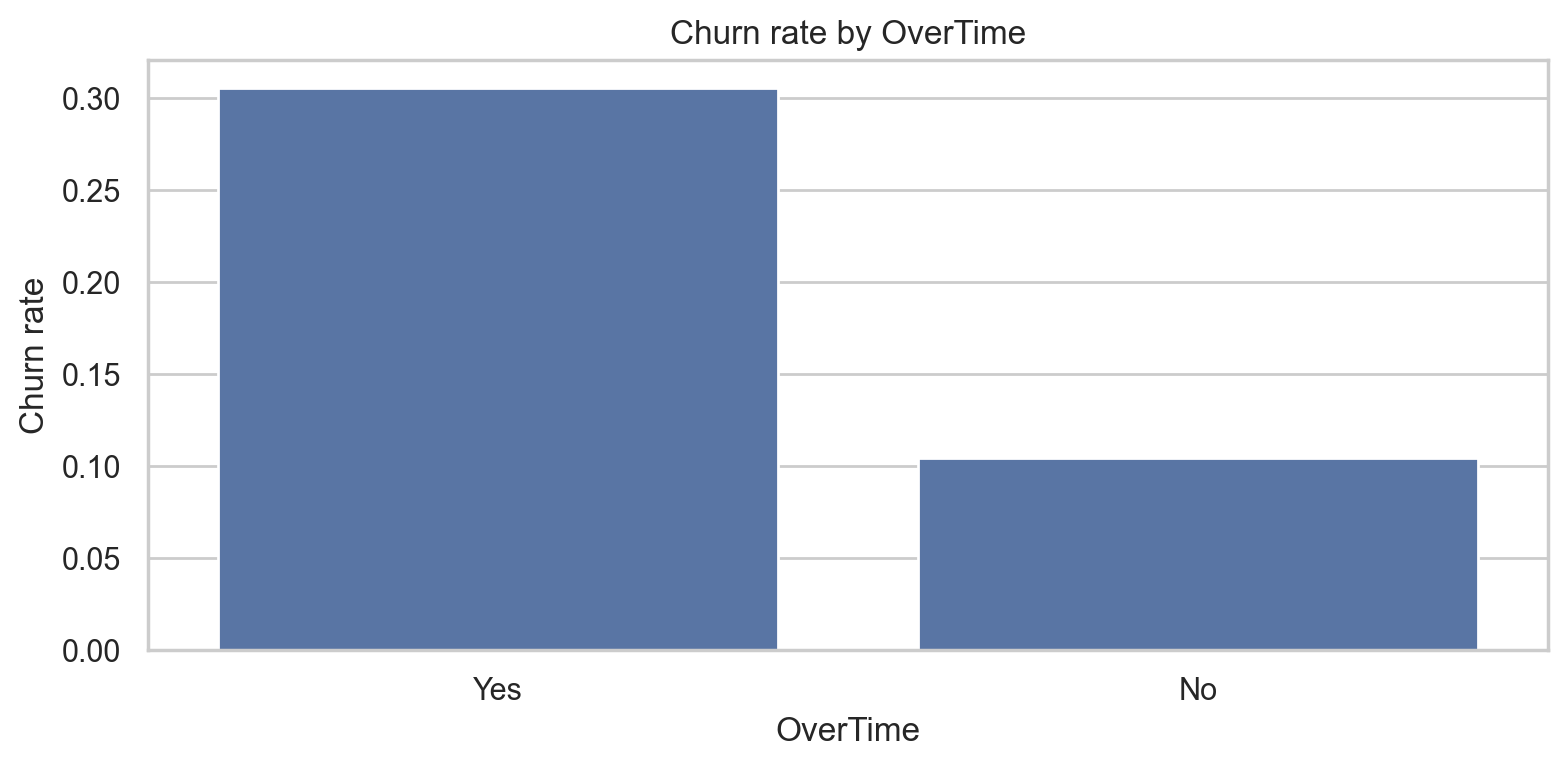
\includegraphics[width=0.6\textwidth]{churn_rate_by_OverTime.png}
  \end{figure}
  
  \vspace{0.4cm}
  \textbf{Quan sát:} Sự chênh lệch khổng lồ. Nhân viên "Yes" (Phải làm thêm giờ) có khả năng rời bỏ cao gấp nhiều lần.
\end{frame}

\begin{frame}{Tỷ lệ nghỉ việc theo JobRole}
  \begin{figure}
    \centering
    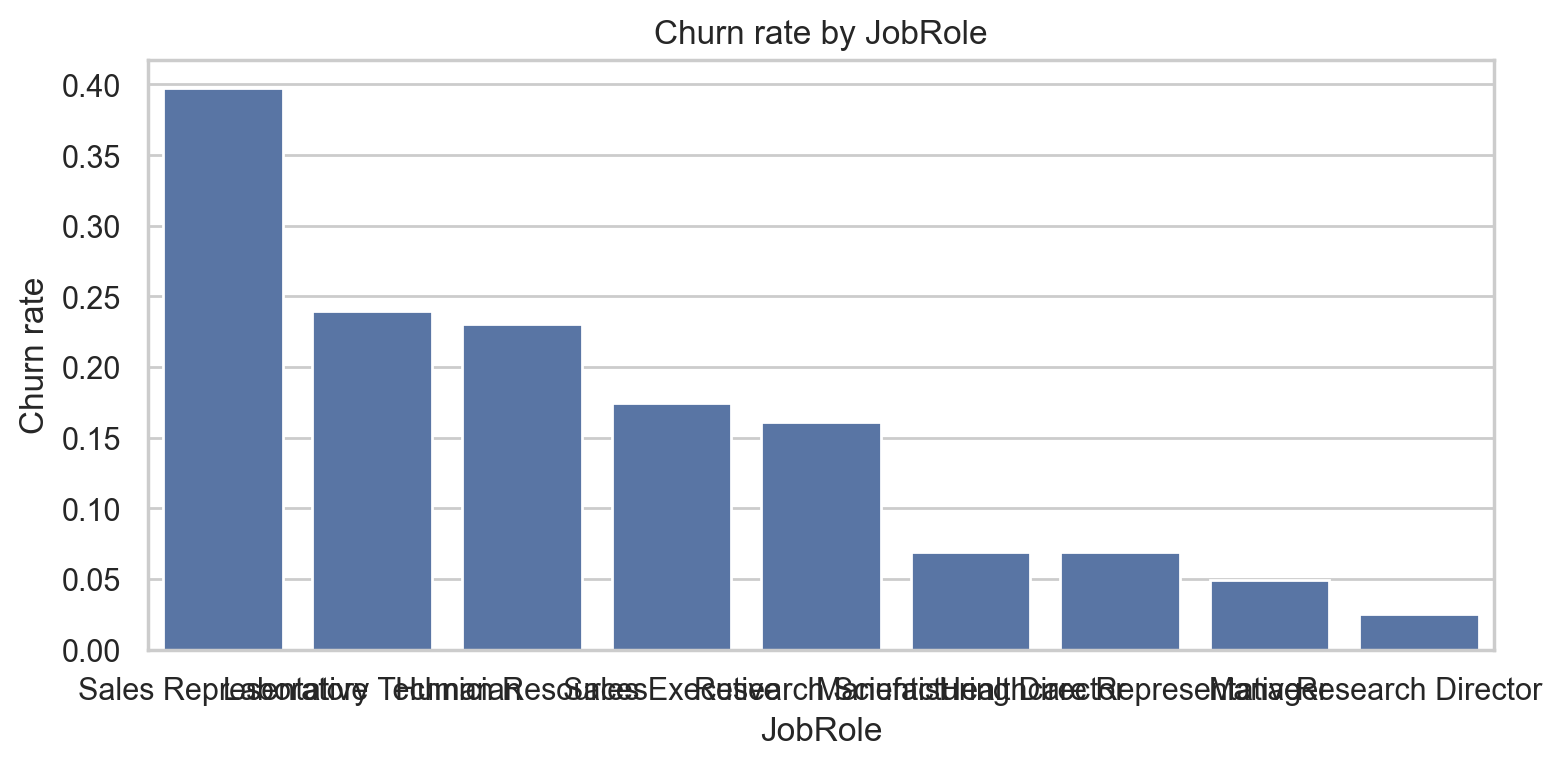
\includegraphics[width=0.6\textwidth]{churn_rate_by_JobRole.png}
  \end{figure}
  
  \vspace{0.4cm}
  \textbf{Quan sát:} \textcolor{mainred}{\textbf{Sales Representative}} và \textbf{Laboratory Technician} đang bị ảnh hưởng luân chuyển nhân sự nghiêm trọng.
\end{frame}

\begin{frame}{Phân phối Age theo trạng thái nghỉ việc}
  \begin{figure}
    \centering
    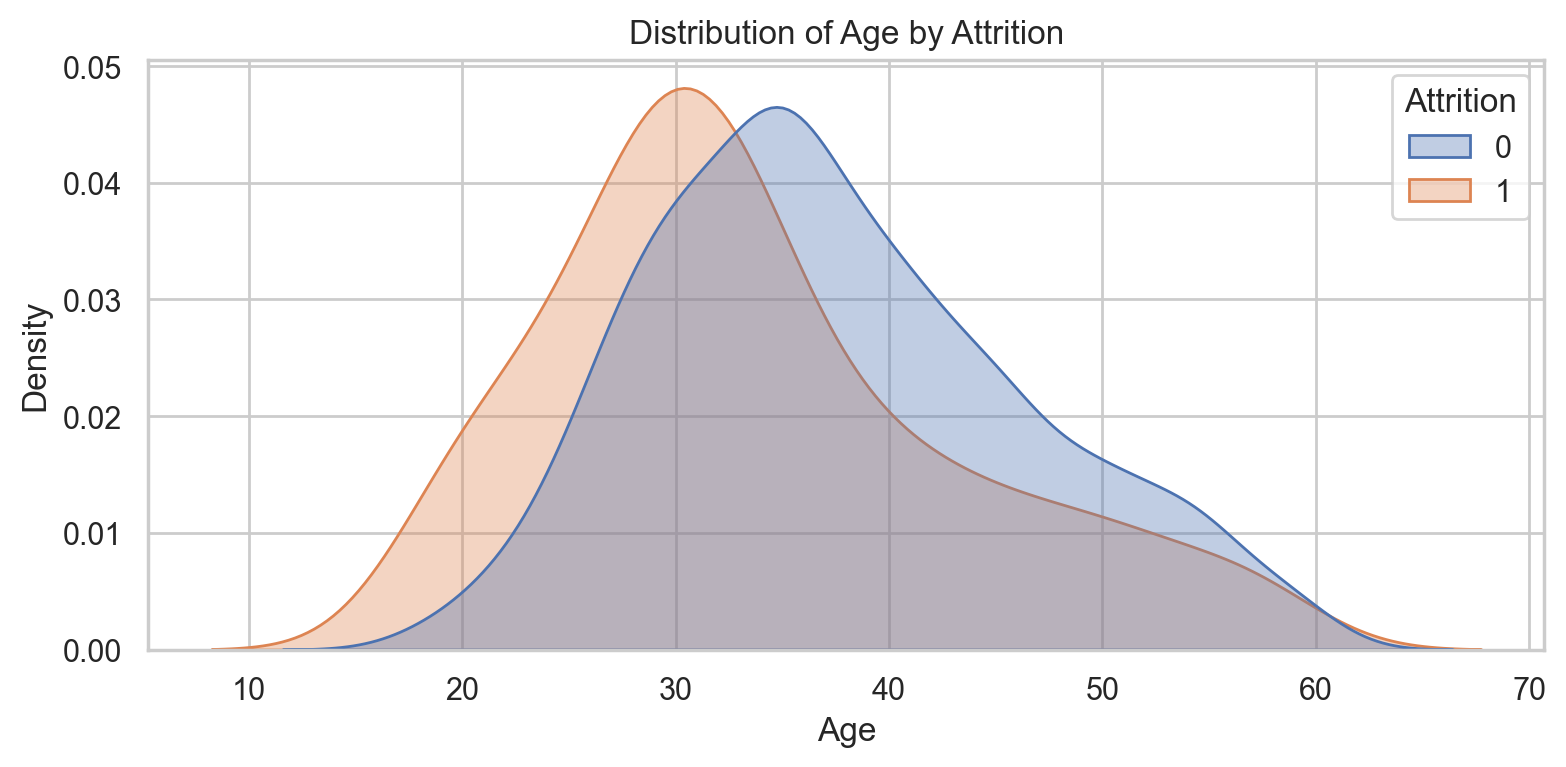
\includegraphics[width=0.65\textwidth]{dist_Age_by_churn.png}
  \end{figure}
  
  \vspace{0.4cm}
  \textbf{Quan sát:} Cá nhân rời công ty thường có \textcolor{mainred}{\textbf{tuổi đời trẻ hơn hẳn}} (đỉnh nhọn tại độ tuổi $<$ 30).
\end{frame}

\begin{frame}{Phân phối MonthlyIncome theo trạng thái nghỉ việc}
  \begin{figure}
    \centering
    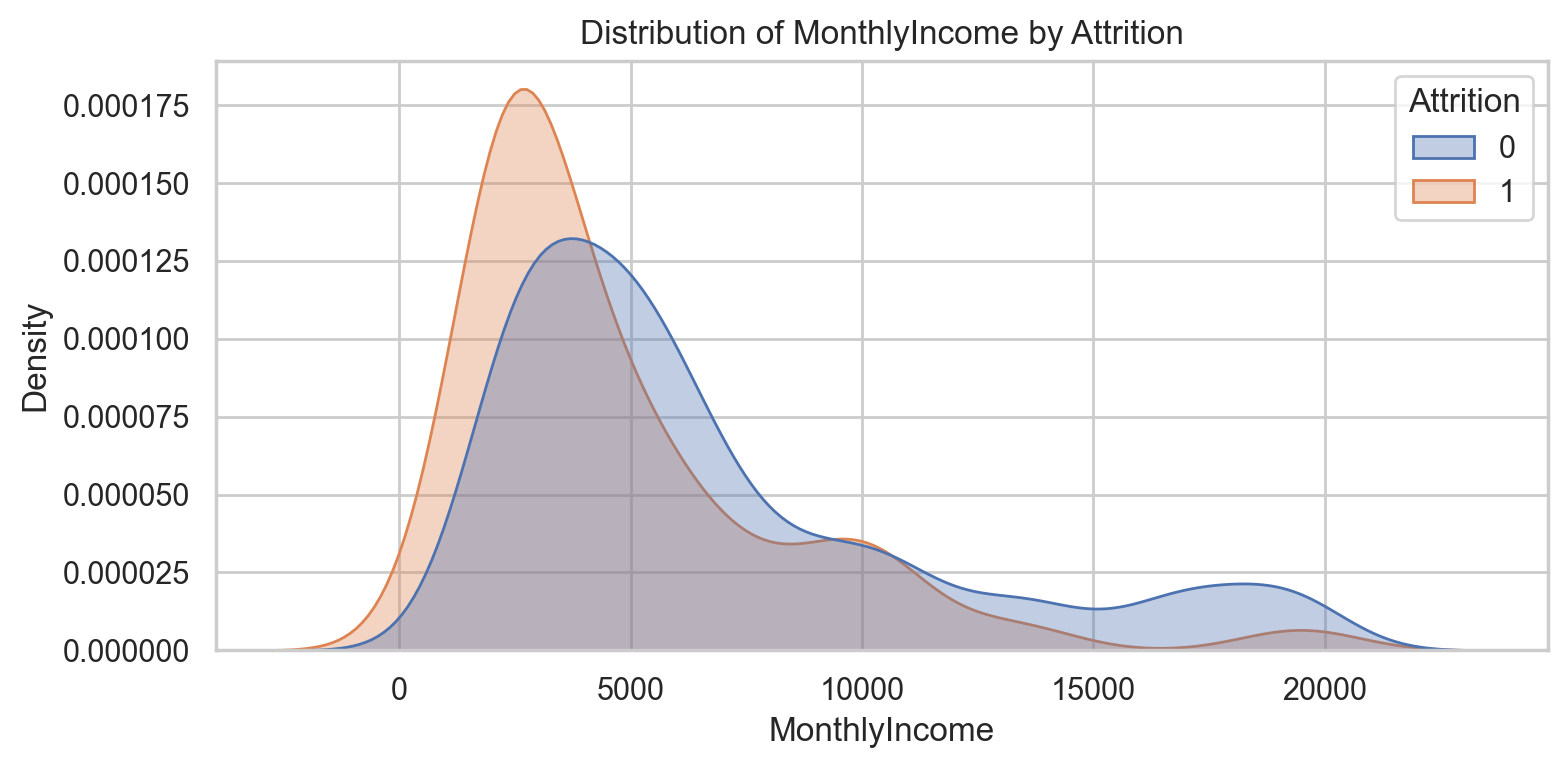
\includegraphics[width=0.65\textwidth]{dist_MonthlyIncome_by_churn.png}
  \end{figure}
  
  \vspace{0.4cm}
  \textbf{Quan sát:} Nhóm nghỉ việc thường rơi vào vùng có thu nhập rất lẹt đẹt. Những người thu nhập cao hầu như ở lại.
\end{frame}

\begin{frame}{Phân phối YearsAtCompany theo trạng thái nghỉ việc}
  \begin{figure}
    \centering
    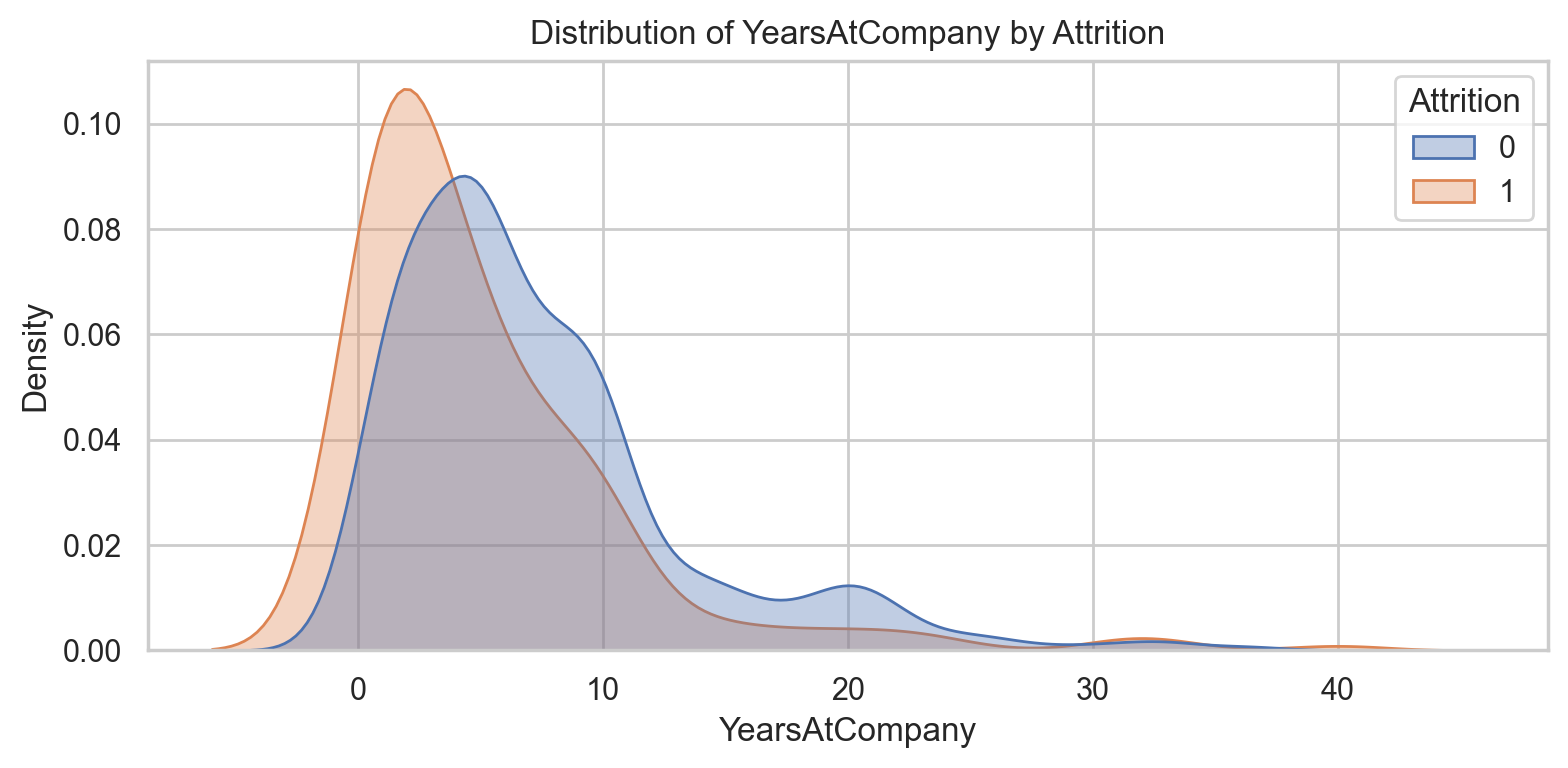
\includegraphics[width=0.65\textwidth]{dist_YearsAtCompany_by_churn.png}
  \end{figure}
  
  \vspace{0.4cm}
  \textbf{Quan sát:} Những năm đầu (dưới 5 năm) là giai đoạn dễ bỏ cuộc nhất. Nếu vượt qua hạn mức đó, xác suất ở lại sẽ cải thiện.
\end{frame}


\section{Đánh giá mô hình}
% Model Evaluation slides
\begin{frame}{Kết quả đánh giá mô hình}
  \centering
  \begin{tabular}{lcc}
    \toprule
    \textbf{Metric} & \textbf{Giá trị} & \textbf{Ý nghĩa} \\
    \midrule
    \textcolor{accentblue}{\textbf{ROC AUC}} & \Large \textbf{0.8031} & Phân biệt tốt, vượt mức ngẫu nhiên xa \\
    \textcolor{accentblue}{\textbf{Recall}} & \Large \textbf{0.6383} & Tóm được khoản 64\% sự cố \\
    Accuracy & 0.7517 & Độ chính xác chung \\
    Precision & 0.3488 & Hiệu suất trong cảnh báo \\
    F1 & 0.4511 & Cân bằng Precision/Recall \\
    \bottomrule
  \end{tabular}
\end{frame}

\begin{frame}{Đánh giá mô hình - Diễn giải}
  \begin{alertblock}{}
    Mô hình ưu tiên \textbf{Recall} (hạn chế bỏ sót nhân tài) - phù hợp với mục tiêu nhân sự
  \end{alertblock}
  
  \vspace{0.4cm}
  \textbf{Ý nghĩa đánh đổi (Trade-off):}
  \begin{itemize}
    \item Nếu mất nhân sự tốn $\gg$ chi phí một buổi trò chuyện, ta cần giữ threshold thấp (như 0.5) để tối đa Recall.
    \item Mô hình chấp nhận một tỷ lệ nhất định báo động ảo (False Positive) để đánh đổi sự an toàn trong quản trị nhân lực.
  \end{itemize}
\end{frame}

\begin{frame}{ROC Curve}
  \begin{figure}
    \centering
    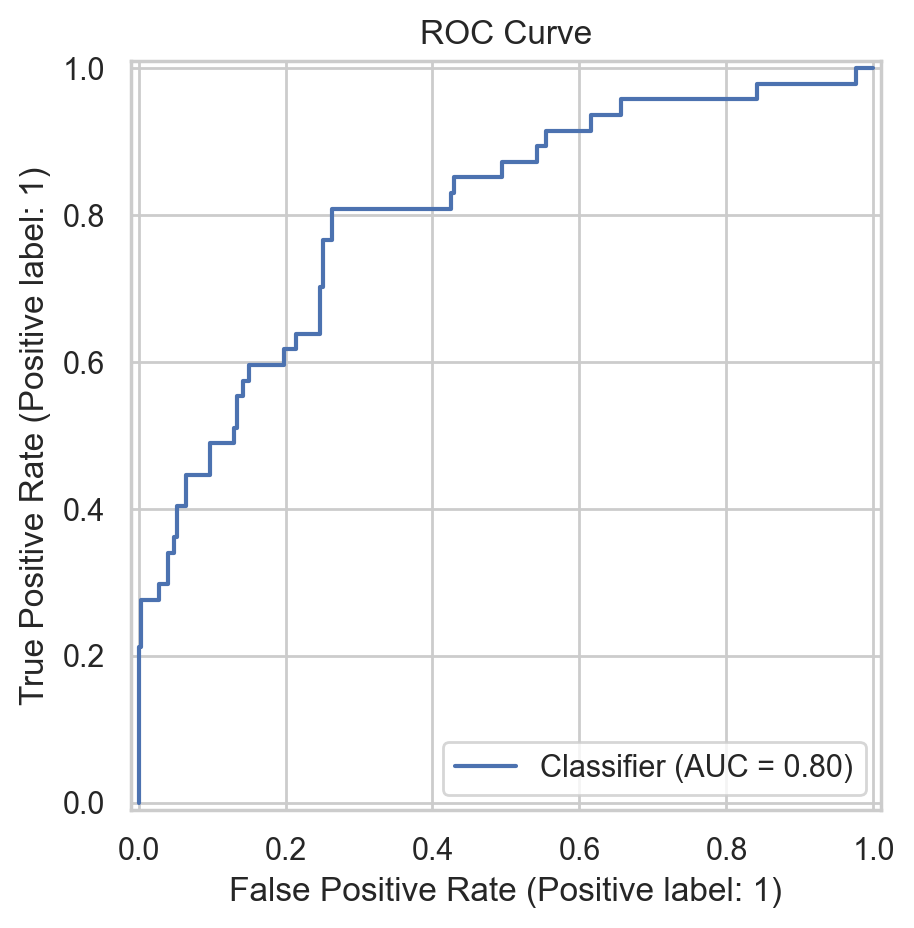
\includegraphics[width=0.65\textwidth]{roc_curve.png}
  \end{figure}
\end{frame}

\begin{frame}{Confusion Matrix}
  \begin{figure}
    \centering
    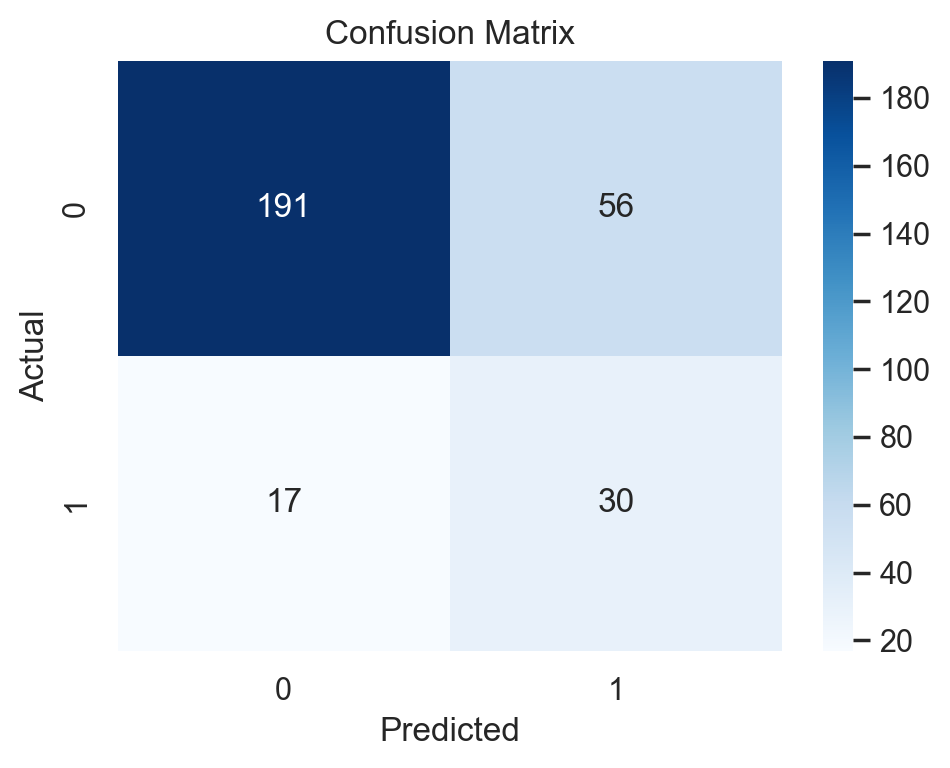
\includegraphics[width=0.55\textwidth]{confusion_matrix.png}
  \end{figure}
\end{frame}

\begin{frame}{Confusion Matrix - Diễn giải}
  \textbf{Phát hiện được khoảng 64\% nguy cơ (Recall = 0.638)}
  
  \vspace{0.4cm}
  \textbf{Thành phần:}
  \begin{itemize}
    \item \textbf{True Positive (TP)}: Nhân viên nghỉ việc được phát hiện và HR có thể cứu vãn
    \item \textbf{False Negative (FN)}: Chảy máu chất xám do hệ thống bỏ sót
    \item \textbf{False Positive (FP)}: Tốn kém dư thừa cho nhân viên không có ý định nghỉ
    \item \textbf{True Negative (TN)}: Quản trị phần đông người tại vị an toàn
  \end{itemize}
\end{frame}


\section{Odds Ratio và diễn giải}
% Odds Ratio slides
\begin{frame}{Odds Ratio (OR) - Diễn giải}
  \textbf{Mô hình logit:}
  \[
  \log\left(\frac{p}{1-p}\right) = \beta_0 + \sum_{j=1}^{d}\beta_j x_j
  \]
  
  \vspace{0.3cm}
  \textbf{Ý nghĩa Odds-Ratio ($OR_j = e^{\beta_j}$):} 
  
  Tăng $x_j$ thêm 1 đơn vị (giữ các biến khác không đổi), odds rủi ro nghỉ việc sẽ \textbf{được nhân với $OR_j$}.
  
  \vspace{0.2cm}
  \begin{itemize}
    \item $OR_j > 1$: Tăng rủi ro (\textbf{Nhân tố áp lực})
    \item $OR_j < 1$: Giảm rủi ro (\textbf{Nhân tố bảo vệ})
  \end{itemize}
\end{frame}

\begin{frame}{Bảng Odds Ratio - Các chỉ số đỉnh cao}
  \footnotesize
  \begin{center}
    \begin{tabular}{@{}lccc@{}}
      \toprule
      \textbf{Feature} & \textbf{OR} & \textbf{95\% CI} & \textbf{p-value} \\
      \midrule
      \textcolor{mainred}{\textbf{OverTime\_Yes}} & \textbf{7.2785} & [4.97, 10.64] & $< 10^{-23}$ \\
      \textcolor{mainred}{\textbf{JobRole\_Sales Rep}} & \textbf{7.1923} & [2.44, 21.19] & 0.0003 \\
      \textcolor{maingreen}{\textbf{EnvironmentSatisfaction}} & \textbf{0.6476} & [0.55, 0.76] & $< 10^{-6}$ \\
      \textcolor{maingreen}{\textbf{JobInvolvement}} & \textbf{0.5891} & [0.46, 0.74] & $< 10^{-4}$ \\
      \textcolor{mainred}{\textbf{BusinessTravel\_Freq}} & \textbf{6.7167} & [2.99, 15.06] & $< 10^{-5}$ \\
      \bottomrule
    \end{tabular}
  \end{center}
  
  \vspace{0.3cm}
  \textit{Ghi chú}: Dummy biến `OverTime\_Yes` lấy `OverTime\_No` làm hệ quy chiếu (baseline).
\end{frame}

\begin{frame}{Forest Plot Odds Ratio}
  \begin{figure}
    \centering
    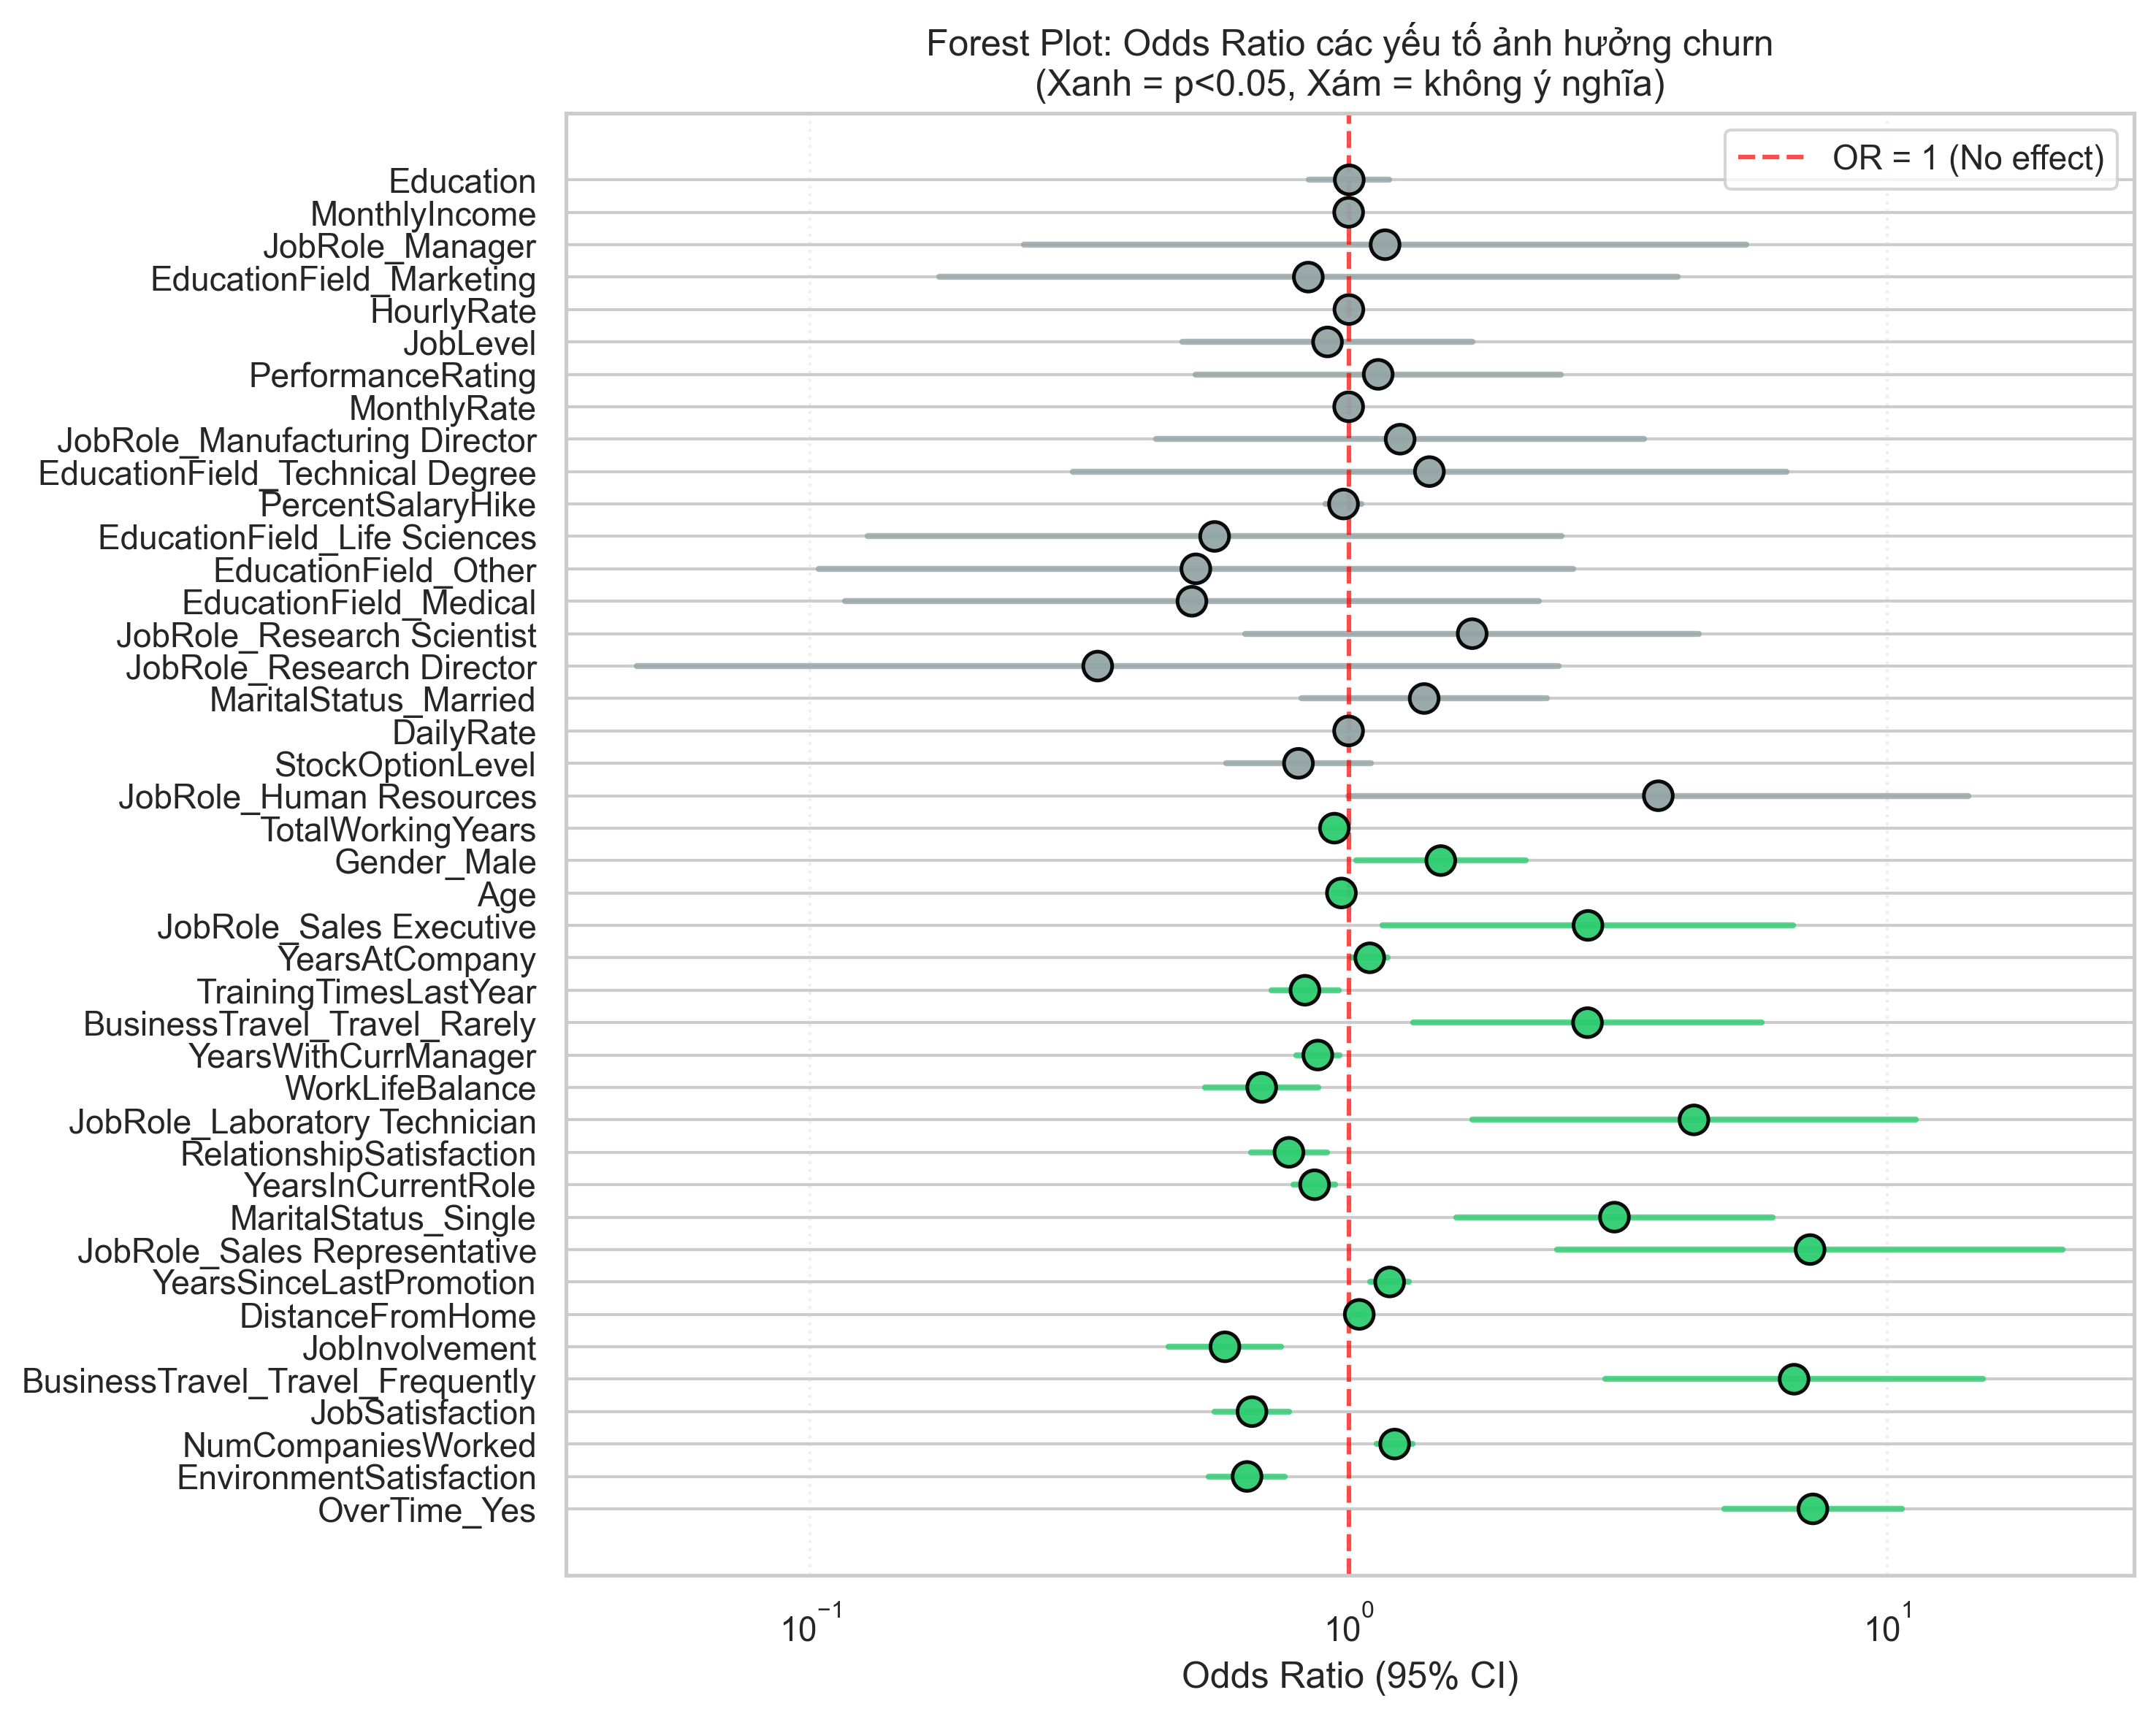
\includegraphics[width=\textwidth,height=0.75\textheight,keepaspectratio]{forest_plot_odds_ratio.png}
  \end{figure}
\end{frame}

\begin{frame}{Yếu Tố Cảnh Báo (OR $\gg$ 1)}
  \textcolor{mainred}{$\uparrow$ Tăng rủi ro nghỉ việc triệt để}
  
  \vspace{0.4cm}
  \begin{itemize}
    \item \textbf{OverTime\_Yes}: OR = 7.28
    \begin{itemize}
      \item Odds nghỉ việc tăng sốc (gấp 7.2 lần) so với người tuân thủ giờ làm hành chính. Áp lực công việc đóng vai trò số 1.
    \end{itemize}
    
    \vspace{0.2cm}
    \item \textbf{JobRole\_Sales Representative}: OR = 7.19
    \begin{itemize}
      \item Nỗi đau của HR ở bộ phận kinh doanh trực tiếp. Áp lực KPI bòn rút nhân viên nặng nề.
    \end{itemize}
    
    \vspace{0.2cm}
    \item \textbf{BusinessTravel\_Travel\_Frequently}: OR = 6.71
    \begin{itemize}
      \item Công tác liên miên đẩy nhân lực đến kiệt sức.
    \end{itemize}
  \end{itemize}
\end{frame}

\begin{frame}{Yếu Tố Bảo Vệ (OR $<$ 1)}
  \textcolor{maingreen}{$\downarrow$ Giảm rủi ro nghỉ việc}
  
  \vspace{0.4cm}
  \begin{itemize}
    \item \textbf{EnvironmentSatisfaction}: OR = 0.64
    \begin{itemize}
      \item Mỗi cấp độ cải thiện môi trường làm giảm 36\% odds rủi ro biến động.
    \end{itemize}
    
    \vspace{0.2cm}
    \item \textbf{JobInvolvement}: OR = 0.58
    \begin{itemize}
      \item Ràng buộc về mặt sự nghiệp và sự đồng hành trong công việc giảm tỷ lệ luân chuyển.
    \end{itemize}
    
    \vspace{0.2cm}
    \item \textbf{WorkLifeBalance}: OR = 0.68
    \begin{itemize}
      \item Đầu tư vào phúc lợi cân bằng cuộc sống có ý nghĩa chiến lược thiết thực. (p-value = 0.002)
    \end{itemize}
  \end{itemize}
\end{frame}


\section{Kết luận}
% Conclusion slides
\begin{frame}{Tổng Kết}
  \textbf{Khái quát Mô hình:}
  
  \vspace{0.3cm}
  \begin{itemize}
    \item \textcolor{accentblue}{\textbf{ROC AUC}}: 0.8031. Quản trị phân loại rủi ro trên 80\%.
    \item \textcolor{accentblue}{\textbf{Gắn nhãn cảnh báo (Recall)}}: 64\%. Đạt được mức trade-off hiệu quả.
  \end{itemize}
  
  \vspace{0.4cm}
  \begin{alertblock}{Đóng góp}
    Báo cáo này loại bỏ phán đoán cảm tính, định lượng và định hình chính xác các lỗ hổng nhân sự, từ đó giảm rủi ro chảy máu chất xám cục bộ.
  \end{alertblock}
\end{frame}

\begin{frame}{Khuyến nghị dành cho Phòng Nhân Sự}
  \textbf{Actionable Recommendations:}
  
  \vspace{0.3cm}
  \begin{enumerate}
    \item \textbf{Can thiệp văn hoá làm ngoài giờ (OverTime)}
    \begin{itemize}
      \item Phải giới hạn mức độ huy động thêm giờ (yếu tố huỷ diệt nhất).
    \end{itemize}
    
    \vspace{0.2cm}
    \item \textbf{Cải tạo chính sách Kinh doanh (Sales Rep) và Công tác (TravelFreq)}
    \begin{itemize}
      \item Khuyến khích thưởng chéo, tăng chế độ công tác phí để bù đắp.
    \end{itemize}
    
    \vspace{0.2cm}
    \item \textbf{Lắng nghe môi trường sở tại (EnvironmentSatisfaction)}
    \begin{itemize}
      \item Quản lý trực tiếp tại điểm làm việc ảnh hưởng tối hậu nhất đến nhân viên. Khảo sát liên tục và chủ động giải quyết xung đột sớm.
    \end{itemize}
  \end{enumerate}
  
  \vspace{0.4cm}
  \textbf{Tái lập quy trình:} \texttt{python scripts/run\_pipeline.py} (Report generation)
\end{frame}


% Thank you slide
\begin{frame}
  \centering
  \vspace{2cm}
  {\Large \textbf{Cảm ơn!}}\\[0.5cm]
  {\large Câu hỏi và thảo luận}
  \vfill
\end{frame}

\end{document}

